\part{Machine Learning}
\label{part:machineLearning}

\chapter{Machine Learning}
\label{chapter:machine_learning}

En este capítulo vamos a hacer un repaso sobre los conceptos asociados al Machine Learning, el aprendizaje y la teoría matemática que involucra. Estas herramientas y conceptos los utilizaremos posteriormente para resolver el problema de detección de anomalías.

\section{Contextualización del aprendizaje}

Para comenzar tenemos que empezar definiendo en que consiste el proceso de aprender sobre unos datos. Supongamos que tenemos un problema en el que tenemos una entrada y una salida, por ejemplo una entrada válida podría ser un vector $x\in \mathbb{R}^d$ y una salida un valor real o un número natural. El problema de aprendizaje intenta estimar una estructura de tipo entrada-salida como la descrita usando únicamente un número finito de observaciones.

Podemos definirlo de forma más general empleando tres conceptos:

\begin{itemize}
	\item Generador: El generador se encarga de obtener las entradas $x\in \mathbb{R}^d$ mediante una distribución de probabilidad $p(x)$ desconocida y fijada de antemano.
	\item Sistema: El sistema es el que produce la salida ``y'' (correcta) para cada entrada $x\in \mathbb{R}^d$ mediante la distribución de probabilidad $p(x|y)$ desconocida y fijada de antemano.
	\item Máquina de aprendizaje: esta es la que va a obtener información de las entradas y salidas conocidas para intentar predecir la salida correcta para una entrada nueva que se nos de. De forma abstracta esta máquina lo que hace es tomar una serie de funciones de un conjunto general de forma que para una entrada dada $x$ la función $f(x,\omega)$ con $\omega \in \Omega$ nos de la salida que corresponde para $x$ donde $\omega$ es una forma de indexar las funciones tomadas para generalizar la salida del conjunto más general de funciones que hemos indicado.
\end{itemize}

El único cabo que hemos dejado sin atar en las definiciones que acabamos de ver es el conjunto de funciones del cual tomaremos algunas para adaptar la máquina de aprendizaje a los datos recibidos. Este conjunto de funciones, que notaremos como $\mathcal{H}$, es de momento la única forma que tenemos de aplicar un conocimiento a priori en la máquina de aprendizaje.

Para finalizar esta breve introducción y poder continuar profundizando vamos a exponer algunos ejemplos de clases de funciones para que podamos visualizar el contexto.

\begin{itemize}
	\item Funciones lineales: En este caso la clase de funciones $\mathcal{H}$ está formada por funciones de la forma $h(x) = w_0 + \sum_{i=1}^{d}x_i w_i$ donde $w\in \mathbb{R}^{d+1}$. Este es el modelo de funciones más clásico.
	\item Funciones trigonométricas: Un ejemplo de una clase de funciones trigonométricas podría ser $f_m(x,v_m,w_m) = \sum_{j=1}^{m-1}(v_j \sin (jx) + w_j \cos (jx)) + w_0$ donde en este caso la entrada es un único valor real. Este tipo de clases de funciones serán útiles en problemas de regresión que luego explicaremos con algo más de detalle aunque sin centrarnos mucho en ello pues no es el objetivo del estudio.
\end{itemize}

\subsection{Objetivo del aprendizaje}

Cuando hablamos de aprendizaje queremos obtener algo de dicho aprendizaje a partir de los datos. Como ya se ha mencionado, intentamos obtener una función de una familia de funciones que aproxime o modele de buena manera la salida del sistema. Por tanto, ese es nuestro objetivo: obtener una función de la familia de funciones que minimice el error.

El problema que enfrentamos es que sólo disponemos de un número finito, por ejemplo $n$, de observaciones de datos y su correspondiente salida. Esto nos va a hacer que no podamos tener una garantía de optimalidad a no ser que tendamos $n$ a infinito. 

Sin embargo si que podemos cuantificar cómo de buena es una aproximación con respecto a otra mediante la función pérdida o error que denotaremos como $L(y,f(x,\omega))$. Esta función nos va a medir la diferencia entre la salida real del sistema y la salida dada por la función $f$ para la entrada $x$ siendo siempre $L(y,f(x,\omega))\geq 0$.

Recordemos además que el Generador obtiene datos mediante una distribución desconocida pero fijada de antemano y que son independientes e idénticamente distribuidos con respecto a la distribución conjunta, es decir:

$$p(x,y) = p(x)p(y|x)$$

Una vez definido todo esto podemos obtener el valor esperado de pérdida o error mediante el funcional

$$R(\omega) = \int L(y,f(x,\omega))p(x,y)dxdy$$

Ahora podemos concretar un poco más lo que entendemos como objetivo del aprendizaje. El objetivo será encontrar una función $f\in \mathcal{H}$ que nos minimice el valor del funcional $R(\omega)$. Pero recordemos que $p(x,y)$ es desconocida para nosotros, por lo que no podemos saber cómo se distribuyen los datos y por tanto el valor del funcional no es calculable para nosotros y por tanto la solución puramente de cálculo no es accesible.

Por tanto, la única forma realmente potente y útil de encontrar una buena aproximación será incorporar el conocimiento a priori que tenemos del sistema. En la sección anterior hemos visto que una forma de incorporar dicho conocimiento es mediante la selección de la clase de funciones, pero además será muy relevante el hecho de cómo los datos son empleados en el proceso de aprendizaje. En este apartado de decisión tendremos que resolver primero la codificación de los datos, el algoritmo empleado y el uso de técnicas como la regularización que veremos después para incorporar nuestro conocimiento en el camino que nos lleve a la solución.

\subsection{Clases de aprendizaje}

El problema de aprendizaje puede ser subdividido a su vez en cuatro clases distintas y que se suelen abordar de forma independiente. Estoss tipos de problemas de aprendizaje son:

\begin{itemize}
	\item Clasificación: El problema de clasificación consiste en identificar y separar instancias de datos según su clase. Por ejemplo podemos dividir a la población mundial en dos clases: sanos y enfermos. Un problema de clasificación podría ser saber identificar estas clases para un conjunto de personas. Los problemas de clasificación más sencillos son aquellos en los que se usan dos únicas clases aunque se puede generalizar la definición del problema a k-clases.
	\item Regresión: El problema de regresión consiste en estimar una función $f: \mathbb{R}^n \rightarrow \mathbb{R}$ a partir de una serie de muestras previas con los valores de $f$. Un problema de regresión podría ser determinar la función que, dados los datos de altura y dimensiones corporales sea capaz de darnos el peso aproximado de la persona.
	\item Estimación de la función de densidad: en este caso no nos interesa la salida que proporciona el sistema, ya sea el valor de una clase o una función real como en el caso de la regresión. En este caso el objetivo del aprendizaje es conseguir la función de densidad $f(x,\omega)$, con $\omega \in \Omega$ los parámetros necesarios de la función de densidad, con la que se distribuyen los datos de entrada del sistema.
	\item Agrupamiento y cuantificación vectorial: El problema de cuantificación vectorial consiste en intentar explicar la distribución de los vectores de entrada mediante puntos clave llamados centroides. De esta forma se podría reducir la complejidad de los datos expresándolos en función de un sistema de generadores menor. El problema de agrupamiento tiene también relación por utilizar la idea de centroide, pero el objetivo es completamente distinto. El objetivo del problema de agrupamiento es intentar conseguir agrupar los datos en clusters, es decir, regiones del espacio en las que se concentran un conjunto de datos. De esta forma intentamos agrupar los datos que mantienen una relación entre sí. Un ejemplo de un problema de cuantificación vectorial podría ser un problema de reducción de dimensionalidad y un ejemplo de problema de agrupamiento podría ser identificar instancias de datos con características comunes.
\end{itemize}

\section{Principios y adaptación del aprendizaje}

Según Vapnik \cite{vapnik_v._nature_nodate} la predicción mediante el aprendizaje se puede dividir en dos fases:

\begin{enumerate}
	\item Aprendizaje o estimación a partir de una muestra.
	\item Predicción a partir de las estimaciones obtenidas.
\end{enumerate}

Estas dos fases se corresponden con los dos tipos de inferencia clásica que conocemos, esto es, inducción y deducción. Traído a este caso el proceso de inducción es aquel que a partir de los datos de aprendizaje o los datos de la muestra que tenemos con la salida que corresponde podemos estimar un modelo. Es decir, estamos sacando el conocimiento de los datos para generar el modelo. El proceso de deducción es aquel que, una vez obtenido el modelo estimado (la generalización) obtenemos una predicción de la salida sobre un conjunto de datos.

Por contra, Vapnik propone un paso que resuelve estas dos fases directamente y que él denomina transducción. Este paso consiste en, dados los datos de entrenamiento obtenemos directamente los valores de salida sin tener que hacer la generalización a un modelo. De esta forma, según Vapnik, podríamos reducir el error que cometemos en la predicción. Este razonamiento tiene sentido, pues estamos omitiendo el paso más complejo del proceso de inducción-deducción.

En resumen esta idea se puede resumir en la siguiente figura:

\begin{figure}[H]
	\centering
	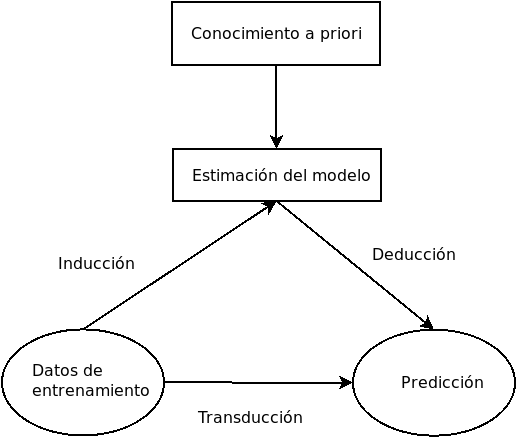
\includegraphics[scale=0.5]{imagenes/induccion_deduccion_transduccion}
	\label{ind_ded_trans}
	\caption{Tipos de inferencia y transduccion \cite[p.~41]{cherkassky_learning_2007}}
\end{figure}

Podemos ver que el conocimiento a priori que tenemos del problema se manifiesta una vez se crea el modelo general, de forma que se emplearía en el paso de la inducción. Ya hemos hablado previamente del conocimiento a priori y cómo incorporarlo al modelo, pero por concretar un poco más podemos añadirlo básicamente de dos formas:

\begin{itemize}
	\item Escogiendo un conjunto de funciones para aproximar la salida del sistema
	\item Añadiendo restricciones o penalizaciones adicionales a dicho conjunto de funciones.
\end{itemize}

En resumen, para poder crear la generalización del modelo de forma única necesitamos:

\begin{enumerate}
	\item Un conjunto de funciones para aproximar la salida.
	\item Conocimiento a priori.
	\item Un principio inductivo, que no es más que una indicación de cómo emplear los datos para llegar a la generalización del modelo.
	\item Un método de aprendizaje, es decir, una implementación del principio inductivo.
\end{enumerate}

En secciones posteriores revisaremos algunos de los principios inductivos más usados pero es importante reseñar la diferencia entre pricipio inductivo y método de aprendizaje. Para un mismo principio inductivo podemos tener varios métodos de aprendizaje, pues podemos escoger diferentes formas de llevarlo a la práctica. Por ejemplo, uno de los principios inductivos más empleados es el ERM o Empirical Risk Minimization, es decir, minimización del error empírico. Podríamos pensar en diferentes formas de utilizar este principio, por ejemplo sólo avanzamos en la creación del modelo si a cada paso que demos minimizamos el error, o por ejemplo vamos avanzando varios modelos a la vez hasta obtener un número de modelos finales de entre los cuales escogeremos aquel que mejor minimice dicho error.

\subsection{Principios inductivos}

Una vez introducido el concepto como hemos hecho en la sección anterior vamos a hacer un breve repaso de los principios más usados y en qué consiste cada uno de ellos.

\subsubsection{Penalización o Regularización}

Imaginemos que tenemos una clase de funciones muy flexible, esto es con un gran número de parámetros libres $f(x,\omega)$ con $\omega \in \Omega$. Vamos a partir de la base del ERM, es decir, minimizar el error empírico. La penalización lo que va a hacer es añadir un factor a la función a minimizar:

$$R_{pen}(\omega) = R_{emp}(\omega) + \lambda \phi [f(x,\omega)]$$

Donde $R_{emp}(\omega)$ es el error empírico con los parámetros $\omega$ y $\phi [f(x,\omega)]$ es un funcional no negativo asociado a cada estimación $f(x,\omega)$. El parámetro $\lambda >0$ es un escalar que controla el peso de la penalización.

El funcional $\phi [f(x,\omega)]$ puede medir lo que creamos conveniente que debemos añadir, es decir, aquí podemos añadir a la minimización algún tipo de medida que nos diga cómo de bien funciona el ajuste de los datos y cómo de bien funciona la información a priori que hemos incluido en el modelo. Pensemos por ejemplo que $\lambda$ fuera un parámetro con un valor muy alto. En este caso la penalización por un mal ajuste de los datos no sería de gran importancia pues lo más conveniente sería minimizar el valor del funcional para no obtener una gran penalización. De esta forma podemos ajustar y dar un poco más de información al error empírico. Por ejemplo, en función del problema, es posible medir la complejidad de la solución mediante el funcional $\phi$ y de esta forma no sólo vamos a obtener una función que ajuste bien los datos, si no que también mantenga una cierta simplicidad para evitar por ejemplo el sobreajuste.

\subsubsection{Reglas de parada anticipada}

Pensemos en un método que vaya aprendiendo de los datos de forma iterativa intentando a cada iteración reducir el error cometido, por ejemplo el ERM. Los métodos o reglas de parada anticipada pueden verse como penalizaciones sobre el algoritmo conforme se va ejecutando. Las reglas de parada anticipada, como su nombre indica lo que preveen es la parada del algoritmo antes de obtener su objetivo teórico. Por ejemplo un algoritmo intenta que el error sea menor que $10^{-6}$ pero para reducirlo desde $10^{-4}$ hasta $10^{-5}$ está consumiendo millones de iteraciones. Si queremos que el tiempo de cómputo penalice lo que podemos hacer es fijar por ejemplo un número máximo de iteraciones que detenga el método aunque no se haya alcanzado esa barrera de error que se preveía.

\subsubsection{Minimización del riesgo estructural o SRM}

Para entender esta filosofía nos ponemos en la situación de que ya sabemos la clase de funciones con la que vamos a aproximar la salida del sistema, por ejemplo hemos escogido la clase de funciones polinómicas. Bajo esta clase de funciones podemos ordenar las funciones por complejidad, entendiendo por complejidad el número de parámetros de la función. Por ejemplo los polinomios de grado $m$ son de menor complejidad que los de grado $m+1$. De esta forma podemos pensar en una estructura de la clase de funciones de la forma:

$$S_0 \subset S_1 \subset S_2 \subset \cdots$$

Este parámetro de complejidad también puede ser un principio a minimizar para intentar conseguir una solución adecuada pero también simple. La generalización de la medida de complejidad para las clases de funciones es la conocida como dimensión VC o dimensión de Vapnik-Chervonenkis.

\subsubsection{Inferencia Bayesiana}

Este principio inductivo se utiliza en el problema de estimación de la función de densidad. El principio es utilizar la conocida fórmula de Bayes para hacer una estimación de la función de densidad empleando el conocimiento a priori que disponemos del problema. La forma en la que se emplea esta fórmula es de la siguiente:

$$P[modelo | datos] = \frac{P[datos | modelo] \cdot P[modelo]}{P[datos]}$$

donde $P[modelo]$ es la probabilidad a priori, $P[datos]$ es la probabilidad de los datos de entrenamiento y $P[datos | modelo]$ es la probabilidad de que los datos estén generados por el modelo.

\subsubsection{Descripción de mínima longitud}

La idea de este principio es la minimización de la longitud que se necesita emplear para describir un modelo y la correspondiente salida. Llamamos l a la longitud total:

$$l = L(modelo) + L(datos | modelo)$$

Esta medida puede ser vista como una medida de complejidad conjunta de todo el modelo.

\section{Regularización}

Por la importancia de este principio inductivo vamos a desarrollarlo un poco más, junto con el concepto de penalización, la selección de los modelos y la relación entre sesgo y varianza. Este último es un concepto muy relevante en cuanto al aprendizaje y que en nuestro caso, al no poseer la clasificación real tendremos que tenerlo en cuenta.

\subsection{Problema de la alta dimensionalidad}

Sabemos que cuando estamos ante un problema de aprendizaje nuestro objetivo es conseguir estimar una función con un número finito de instancias de una muestra ya con la salida. Al tener un número finito de elementos en la muestra ya sabemos que no podemos garantizar que la respuesta sea la óptima o correcta, pero además debemos pensar que a mayor regularidad del conjunto de funciones empleado debemos tener una densidad suficiente de puntos para compensar dicha regularidad. Este problema es conocido como la maldición de la dimensionalidad (curse of dimensionality). El problema es que cuanto mayor sea la dimensionalidad considerada más difícil es poder tener esa alta densidad de datos que se requieren para funciones muy regulares.

Este problema que conlleva la alta dimensionalidad proviene de la geometría de los espacio con alta dimensionalidad. A medida que incrementamos la dimensionalidad el espacio se ve cada vez con más aristas o picos. Podemos pensar en un cubo para el espacio tridimensional y a medida que aumentamos la dimensión incorporamos más aristas y vértices. Podemos resumir en 4 propiedades de los espacio con alta dimensionalidad que causan este problema:

\begin{enumerate}
	\item La densidad disminuye exponencialmente al aumentar el número de dimensiones. Supongamos que tenemos una muestra de $n$ puntos en $\mathbb{R}$. Para poder tener la misma densidad en un espacio $d$-dimensional $\mathbb{R}^d$ necesidamos $n^d$ puntos.
	\item Cuanto mayor dimensionalidad tenga el conjunto de datos mayor lado se necesita para que un hipercubo contenga el mismo porcentaje del conjunto que con una menor dimensionalidad. Imaginemos que tenemos un conjunto $d$-dimensional en el que tenemos la muestra dentro de un hipercubo unidad. Si quisiéramos abarcar un porcentaje $p\in [0,1]$ necesitaríamos un cubo de lado $e_d (p) = p^{\frac{1}{d}}$. Como se puede observar a mayor dimensionalidad y $p$ constante el lado es cada vez mayor. Esta idea es fácilemente entendible si observamos la siguiente figura:
	
	\begin{figure}[H]
		\centering
		\label{radio_alta_dimensionalidad}
		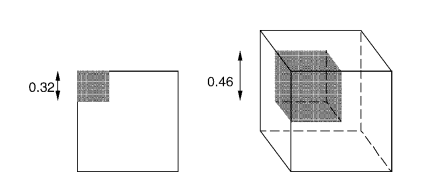
\includegraphics[scale=0.6]{imagenes/radio_alta_dimensionalidad}
		\caption{Para 2 dimensiones necesitamos menor lado que para 3 dimensiones. \cite[p.~64]{cherkassky_learning_2007}}
	\end{figure}
	\item Casi todo punto está más cerca de un borde que de otro punto. Pensemos en un conjunto de datos con $n$ puntos distribuidos de forma uniforme en una bola $d$-dimensional de radio unidad. Para este conjunto de datos, según \cite{hastie_t._elements_nodate}, la distancia media entre el centro de la distribución y los puntos más cercanos a dicho centro se mide bajo la fórmula:
	
	$$D(d,n) = (1-\frac{1}{2}^{1/n})^{1/d}$$
	
	Si en esta fórmula tomamos por ejemplo $n=200$ y $d=10$ el resultado es $D(10,200) \approx 0.57$. Esto significa que los puntos más cercanos al centro de la distribución están más cerca de los bordes que del centro.
	\item Casi todo punto es una anomalía sobre su propia proyección. Si pensamos de nuevo en la idea de los vértices y aristas en espacio de alta dimensionalidad y pensamos en que, según el punto anterior, cada vez que aumenta la dimensionalidad los puntos están más cerca de los bordes entonces no es extraño pensar que los puntos a medida que aumenta la dimensionalidad están más distantes del resto de puntos. Esto intuitivamente (ya que aún no hemos visto la definición formal de anomalía) nos guía a pensar que vistos los puntos en sus propios entornos éstos serán anomalías comparados con el resto.
	
	\begin{figure}[H]
		\centering
		\label{espacio_alta_dimension}
		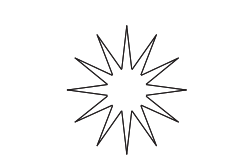
\includegraphics[scale=0.6]{imagenes/espacio_alta_dimension}
		\caption{Forma conceptual de un espacio de alta dimensionalidad.\cite[p.~64]{cherkassky_learning_2007}}
	\end{figure}

	Conceptualmente podemos imaginarlo con esta forma de picos, con lo que si tenemos los datos apiñados en dichos picos o extremos el resto de datos que estén en picos diferentes distan tanto del que estamos considerando que no podemos afirmar que tengan ninguna relación entre sí.
\end{enumerate}

Estos puntos hemos de recordar que van referidos al conjunto de datos y no a las funciones que estamos considerando para representar la salida del sistema. Si estamos considerando la complejidad de las funciones la dimensionalidad no es una buena medida. Sabemos de la existencia de teoremas de aproximación de funciones como por ejemplo el Teorema de Superposición de Kolmogorov-Arnold.

\begin{teorema}[Teorema de Superposición de Kolmogorov-Arnold]
	Sea $f$ una función continua de varias variables $f:X_1 \times ... \times X_n \rightarrow \mathbb{R}$, entonces existen funciones $\Phi_q : \mathbb{R}\rightarrow \mathbb{R}$ y $\phi_{q,p} : X_p \rightarrow [0,1]$ tales que $f$ se puede expresar como:
	
	$$f(x) = f(x_1, ..., x_n) = \sum_{q=0}^{2n}\Phi_q ( \sum_{p=1}^{n}\phi_{q,p}(x_p))$$
\end{teorema}

Este Teorema argumenta perfectamente que la complejidad que le damos a los datos por tener una alta dimensionalidad no es transferible a las funciones pues podemos expresar funciones de varias variables como combinación de funciones de una sola variables. En otras palabras no podemos argumentar que la complejidad de funciones univariantes sea mayor o menor que la de funciones multivariantes.

\subsection{Aproximación de funciones}

Como ya hemos dicho en la introducción queremos aproximar una función salida del sistema dentro de una familia de funciones. Este campo no es nuevo, tenemos como herramientas una serie de Teoremas relacionados con la aproximación de funciones como el Teorema de Kolmogorov enunciado anteriormente o el Teorema de aproximación de Weierstrass.

La versión más simple del Teorema de Weierstrass es la de funciones reales definidas en intervalos cerrados, veamos un repaso de estos Teoremas para hacer un esquema de la aproximación de funciones.

\begin{teorema}[Teorema de aproximación de Weierstrass]
	Supongamos que $f:[a,b] \rightarrow \mathbb{R}$ es una función continua. Entonces $\forall \epsilon >0$, $\exists p$ un polinomio tal que $\forall x\in [a,b]$ tenemos que $|f(x)-p(x)|<\epsilon$.
\end{teorema}

En otras palabras, podemos aproximar las funciones continuas reales definidas en un intervalo cerrado con el error que queramos en un punto mediante polinomios. Además tenemos versiones más generales aún como el Teorema de Stone-Weierstrass para funciones reales, para espacios localmente compactos y para el espacio de los complejos.

Estas aproximaciones son más sencillas en términos de la complejidad de la clase de funciones, pero tenemos aproximaciones muy famosas, como por ejemplo la serie de Fourier.

\begin{definicion}[Serie de Fourier]
	Si tenemos una función $f:\mathbb{R} \rightarrow \mathbb{R}$ integrable en el intervalo $[t_0 - \frac{T}{2}, t_0 + \frac{T}{2}]$ entonces se puede obtener el desarrollo en serie de Fourier de $f$ en dicho intervalo. Si $f$ es periódica en toda la recta real la aproximación será válida en todos los valores en los que esté definida.
	
	$$f(t) \approx \frac{a_0}{2} + \sum_{n=1}^{\infty}[a_n \cos (\frac{2n\pi}{T}t) + b_n\sin (\frac{2n\pi}{T}t)]$$
	
	Donde $a_0, a_n$ y $b_n$ son los coeficientes de la serie de Fourier que tienen la forma:
	
	$$a_0 = \frac{2}{T}\int_{-\frac{T}{2}}^{\frac{T}{2}}f(t)dt$$
	
	$$a_n = \frac{2}{T}\int_{-\frac{T}{2}}^{\frac{T}{2}}f(t) cos(\frac{2n\pi}{T}t)dt$$
	
	$$b_n = \frac{2}{T}\int_{-\frac{T}{2}}^{\frac{T}{2}}f(t) \sin (\frac{2n\pi}{T}t)dt$$
\end{definicion}

Como podemos ver hemos introducido dos conocidas formas de aproximar funciones, una con funciones polinómicas y otra con funciones trigonométricas. Vamos a dividir en dos los tipos de  aproximación que podemos tener para el problema de aprendizaje.

\begin{enumerate}
	\item Aproximaciones universales: son aquellas en las que se establece que cualquier función continua puede ser aproximada por otra función de otra clase con el error que queramos. En este grupo podríamos meter a los dos teoremas que hemos dado previamente. Dentro de este grupo podemos tener diferentes tipos de aproximaciones en función de la familia de funciones que escojamos como aproximaciones. Por ejemplo en los dos teoremas previos hemos cogido las clases de funciones polinómicas y trigonométricas pero podríamos haber tomado otras clases diferentes.
	\item Aproximaciones inexactas: son aquellas en las que no podemos tener una aproximación como las que hemos dado en los teoremas previos, si no que proveen de una aproximación de peor calidad.
\end{enumerate}

\subsection{Penalización o control de la complejidad}

Ya hemos discutido brevemente en la sección de principios inductivos la complejidad y cómo penalizarla. Vamos a ver qué elementos queremos controlar con la penalización:

\begin{enumerate}
	\item La clase de funciones con la que vamos a hacer la aproximación. Tenemos que decidir si escoger una clase tan amplia que nos aseguremos que abarque la solución seguro pero penalicemos la complejidad de la elección o queremos una clase de funciones más ajustada.
	\item Tipo de funcional de penalización. Tenemos que escoger entre los distintos tipos de penalización que queremos. Esto se reduce a escoger entre dos tipos de penalización: paramétrica y no paramétrica. La primera de ellas se basa en estudiar la suavidad del ajuste junto con el número de parámetros que requiere la aproximación mientras que la segunda intenta estudiar lo mismo, es decir la suavidad del ajuste, sin medir los parámetros de la clase de funciones. En este punto se puede incorporar el conocimiento a priori del problema.
	\item Método con el que queremos minimizar la penalización. Este apartado está relacionado con los métodos que tenemos de aprender de los datos y el objetivo será intentar hallar una forma eficiente de minimizar tanto el error de la aproximación como la propia penalización.
	\item Control de la complejidad. Como hemos dicho antes el control de la complejidad no es algo sencillo y habrá que escoger la mejor manera de medir dicha complejidad. En secciones posteriores veremos medidas de complejidad como la dimensión de Vapnik-Chervonenkis.
\end{enumerate}

Veamos brevemente la distinción que hemos hecho entre la penalización paramétrica y no paramétrica.

\subsubsection{Penalización paramétrica}

Supongamos que tenemos un conjunto de funciones $f(x,\omega)$ con $\omega \in \Omega$ donde $\Omega$ es el conjunto de parámetros de la forma $\omega = (\omega_0 , ... , \omega_m)$. Como la aproximación viene definida por el parámetros $\omega$ entonces podemos definir también la penalización asociada a dicha selección de parámetros.

Vamos a ver los ejemplos de las penalizaciones más empleadas de este tipo.

\begin{itemize}
	\item Ridge: $\phi_r (\omega_m) = \sum_{i=0}^{m}\omega_i^2$
	\item Selección de subconjunto: $\phi_s (\omega_m) = \sum_{i=0}^{m}\chi (\omega_i \neq 0)$
	\item Bridge: $\phi_p (\omega_m) = \sum_{i=0}^{m}|\omega_i|^p$
	\item Decaimiento de peso: $\phi_q (\omega_m) = \sum_{i=0}^{m}\frac{(\omega_i / q)^2}{1+(\omega_i / q)^2}$ 
\end{itemize}

\subsubsection{Penalización no paramétrica}

En primer lugar vamos a definir la transformada de Fourier de una función para poder definir el funcional de penalización. 

\begin{definicion}[Transformada de Fourier]
	Sea $f$ una función integrable Lebesgue, $f\in L(\mathbb{R})$. Se define la transformada de Fourier de $f$ como la función:
	
	$$\mathcal{F}\{f\} : \xi \rightarrow \hat{f}(\xi) := \int_{-\infty}^{\infty}f(x)e^{-2\pi i\xi x}dx$$
\end{definicion}

Recordemos brevemente las propiedades de la transformada de Fourier.

\begin{itemize}
	\item La transformada de Fourier es un operador lineal: $\mathcal{F}\{a\cdot f + b\cdot g\} = a\mathcal{F}\{f\} + b\cdot \mathcal{F}\{g\}$
	\item $\mathcal{F}\{f(at)\}(\xi) = \frac{1}{|a|}\cdot \mathcal{F}\{f\}(\frac{\xi}{a})$
	\item $\mathcal{F}\{f(t-a)\}(\xi) = e^{-\pi i\xi a}\cdot \mathcal{F}\{f\}(\xi)$
	\item $\mathcal{F}\{f\}(\xi -a) = \mathcal{F}\{e^{\pi iat}f(t)\}(\xi)$
	\item $\mathcal{F}\{f'\}(\xi) = 2\pi i\xi \mathcal{F}\{f\}(\xi)$
	\item $\mathcal{F}\{f\}'(\xi) = \mathcal{F}\{(-it)\cdot f(t)\}(\xi)$
\end{itemize}

Habiendo recordado esto podemos definir el funcional de penalización no paramétrica. Este funcional mide la suavidad del ajuste de la función gracias a que se puede medir, mediante la transformada de Fourier, la ondulación de la función. Por tanto el funcional no paramétrico que se propone es:

$$\phi [f] = \int_{\mathbb{R}^d}\frac{|\hat{f}(s)|^2}{\hat{G}(s)}ds$$

Donde $\hat{f}$ indica la transformada de Fourier de la función $f$ y $\frac{1}{\hat{G}}$ es la transformada de Fourier de una función de filtro de paso alto. Es en esta proposición de filtro donde se añade el conocimiento a priori del problema. Por ejemplo pudiera ser interesante en alguna aplicación práctica tener un funcional invariante frente a rotaciones de funciones.

\subsection{Equilibrio entre el sesgo y la varianza}

Este enfoque es muy utilizado en el estudio del error, dividiéndolo en sesgo y varianza para hacer un mejor estudio del mismo y poder enfrentar ambos con varios métodos. Este estudio del caso clásico no es válido (o al menos no del todo) para problemas no supervisados como es nuestro caso. Vamos a hacer una adaptación de esta teoría para que pueda encajar en nuestro caso de estudio.

Tenemos que tener en cuenta que no conocemos la salida real del sistema en el caso de detección de anomalías, es decir, no sabemos estimar con certeza el sesgo y la varianza y por tanto el error que cometemos. En primer lugar vamos a ver una pequeña adaptación de la notación al caso de detección de anomalías para poder hacer un estudio enfocado.

Vamos a notar por $X_1 , ... , X_n$ los datos de test y $\mathcal{D}$ como conjunto de datos de entrenamiento. Además vamos a considerar que existe una función $f$ que nos da la etiqueta real de un dato, esto es, si es o no una anomalía. Por tanto podemos decir que la auténtica etiqueda de un dato es $y_i = f(X_i)$. Además nosotros estaremos usando un modelo ya escogido por nosotros para predecir la etiqueta de un dato de test, esto es $g(X_i, \mathcal{D})\approx y_i+\beta$ donde $\beta$ es un cierto error.

Una vez conocida esta notación podemos definir el error medio al cuadrado como:

$$MSE = \frac{1}{n}\sum_{i=1}^{n}\{y_i - g(X_i, \mathcal{D})\}^2$$

Y podemos definir también el valor esperado del error medio al cuadrado como:

$$E[MSE] = \frac{1}{n} \sum_{i=1}^{n}E[\{y_i - g(X_i, \mathcal{D}\}^2]$$

Una vez definido el $MSE$ esperado podemos desarrollar un poco el cálculo para poder obtener el error y la varianza que esperamos.

En primer lugar podemos escribirlo como:

$$E[MSE] = \frac{1}{n}\sum_{i=1}^{n}E[\{ (y_i-f(X_i)) + (f(X_i) - g(X_i,\mathcal{D})) \}^2]$$

Aquí solo hemos restado y sumado $f(X_i)$, ahora si recordamos que $y_i = f(X_i)$ entonces podemos igualar el primero de los paréntesis a $0$ y por tanto nos queda:

$$E[MSE] = \frac{1}{n}\sum_{i=1}^{n}E[\{ f(X_i) - g(X_i, \mathcal{D}) \}^2]$$

Si seguimos descomponiendo podemos sumar y restar $E[g(X_i, \mathcal{D})]$ con lo que nos quedaría:

$$E[MSE] = \frac{1}{n}\sum_{i=1}^{n}E[\{ f(X_i) - E[g(X_i, \mathcal{D})] \}^2]$$

$$ + \frac{2}{n}\sum_{i=1}^{n}\{ f(X_i) - E[g(X_i, \mathcal{D})] \}\cdot \{ E[g(X_i, \mathcal{D})] - E[g(X_i, \mathcal{D})] \}$$

$$ + \frac{1}{n}E[\{ E[g(X_i, \mathcal{D}) - g(X_i, \mathcal{D})] \}^2]$$

Como es claro, el segundo término da cero por lo que nos queda al final:

$$E[MSE] = \frac{1}{n} \sum_{i=1}^{n}E[\{ f(X_i) - E[g(X_i, \mathcal{D})] \}^2] + \frac{1}{n}\sum_{i=1}^{n}E[\{ E[g(X_i, \mathcal{D})] - g(X_i, \mathcal{D}) \}^2]$$

$$=\frac{1}{n}\sum_{i=1}^{n}\{ f(X_i) - E[g(X_i, \mathcal{D})] \}^2 + \frac{1}{n}\sum_{i=1}^{n}E[\{ E[g(X_i, \mathcal{D})] - g(X_i, \mathcal{D}) \}^2]$$

Si reconocemos cada uno de los términos, en primer lugar el primero de ellos es el sesgo al cuadrado y el segundo la varianza, por lo que finalmente lo que hemos obtenido es:

$$E[MSE] = sesgo^2 + varianza$$

El dilema que se nos plantea es el siguiente: si tomamos modelos con un bajo sesgo en la estimación de los parámetros entonces tendremos una alta varianza y viceversa. Esto significa que no podemos con el conocimiento del que disponemos disminuir tanto el sesgo como la varianza a la vez. Es esta propiedad la que se conoce como la compensación entre sesgo y varianza.

\section{Teoría estadística del aprendizaje}

En esta sección vamos a hacer un repaso por la teoría del aprendizaje, en concreto la teoría desarrollada por Vapnik-Chervonenkis. Esta teoría se basa o tiene como pilares cuatro puntos:

\begin{enumerate}
	\item Condiciones para la consistencia del principio ERM o minimización del error empírico.
	\item Cotas en la capacidad de generalización de las máquinas de aprendizaje.
	\item Principios de inferencia sobre muestras finitas.
	\item Métodos constructivos para implementar los principios inductivos ya expuestos.
\end{enumerate}

Durante el desarrollo de esta sección haremos un repaso de estos cuatro puntos para dar el broche final a esta sección y poder realizar la primera de las definiciones de anomalía.

\subsection{Condiciones para la convergencia y consistencia del ERM}

En el problema de aprendizaje disponemos de una muestra en la que tenemos los propios datos de entrada y la salida del sistema. Denotemos a estos elementos por $z=(x,y)$ donde $x$ son los datos de entrada e $y$ la salida del sistema. Por tanto la muestra que se nos da es un conjunto $Z_n = \{ z_1 , ... , z_n \}$. Estos datos están generados como ya sabemos mediante una función de densidad desconocida $p(z)$. Sobre este esquema tenemos una serie de funciones de pérdida y un funcional de pérdida. El objetivo es encontrar dicha función de pérdida $Q(z,\omega )$ que minimice dicho funcional:

$$R(\omega) = \int Q(z,\omega) p(z)dz$$

Por tanto si tenemos la función de pérdida podemos definir el error empírico como:

$$R_{emp}(\omega) = \sum_{i=1}^{n}Q(z_i, \omega)$$

Donde $\omega$ son los parámetros escogidos para el modelo.

Para poder estudiar la consistencia del ERM primero debemos definir formalmente dicha propiedad. Denotamos por $R_{emp}(\omega_n^*)$ el valor del error empírico con la función de pérdida $Q(z,\omega_n^*)$ que minimiza el error empírico para el conjunto de entrenamiento $Z_n$. Denotemos además por $R(\omega_n^*)$ el verdadero valor (desconocido) del error para la función de pérdida. Como se puede ver estos valores dependen del tamaño del conjunto de entrenamiento $n$, podemos por tanto estudiar cómo se comportan estos errores cuando aumentamos el tamaño del conjunto de entrenamiento. Es aquí donde entra la definición de consistencia del ERM. Decimos que es consistente si la sucesión de errores reales y empíricos convergen en probabilidad al mismo límite $R(\omega_0) = \min_{\omega} R(\omega)$. Es decir:

$$R(\omega_n^*) \rightarrow R(\omega_0) \ cuando \ n\rightarrow \infty$$
$$R_{emp}(\omega_n^*) \rightarrow R(\omega_0) \ cuando \ n\rightarrow \infty$$

Para poder asegurar esta propiedad sobre el ERM tenemos el conocido como Teorema Clave de la Teoría del Aprendizaje de Vapnik y Chervonenkis.

\begin{teorema}[Teorema Clave de la Teoría del Aprendizaje]
	Para funciones de pérdida acotadas el principio inductivo de minimización del error empírico es consistente sí y sólo si el error empírico converge uniformemente al valor real del error en el siguiente sentido:
	
	$$\lim\limits_{n\rightarrow \infty} P[\sup_{\omega}|R(\omega) - R_{emp}(\omega)|>\epsilon] = 0 \ , \ \forall \epsilon >0$$
\end{teorema}

Cabe recalcar que estas condiciones de consistencia dependen de las propiedades de la clase de funciones elegida. No podemos pretender escoger como clase de aproximación una muy general y seguir manteniendo las condiciones de consistencia del ERM. Aún así el teorema nos está dando condiciones generales para la consistencia del ERM pero son abstractas y no fácilmente aplicables en la práctica. Para ello vamos a estudiar las condiciones de convergencia de ERM que sí serán aplicables en la implementación de algoritmos.

Vamos ahora a particularizar el estudio en el caso de clasificación binaria por ser la materia de estudio que nos ocupa, pues al final tendremos que clasificar instancias en anómalas o no anómalas. Ahora las funciones de pérdida $Q(z,\omega)$ son funciones de pérdida indicadoras. Vamos a notar por $N(Z_n)$ el número de dicotomías que se pueden tener con la clase de funciones elegidas. Esto es el número de formas de clasificar los datos en las dos clases existentes.

Una vez actualizada nuestra notación podemos definir la entropía aleatoria como $H(Z_n) = \ln N(Z_n)$. Esta cantidad es una variable aleatoria dependiente de los valores de entenamiento $Z_n$, podemos definir ahora la entropía de Vapnik-Chervonenkis como el valor medio o esperado de la entropía aleatoria:

$$H(n) = E[\ln N(Z_n)]$$

Esta medida es una cuantificación de la diversidad del conjunto de funciones indicadoras que nos pueden separar los datos en ambas clases.

Por último vamos a definir la función de crecimiento que nos va a permitir hacer cotas y llegar a la condición necesaria y suficiente para la convergencia del ERM. Definimos la función de crecimiento como:

$$G(n) = \ln \max_{Z_n} N(Z_n)$$

Donde aquí estamos notando el máximo número de dicotomías sobre todas las posibles muestras existentes de tamaño $n$. Es más, como el máximo número de formas de dividir un conjunto de tamaño $n$ en dos clases es $2^n$ entonces podemos afirmar que $G(n)\leq n\ln (2)$.

Por último y para completar la cadena de desigualdades que buscamos vamos a definir la entropía reforzada de Vapnik-Chervonenkis:

$$H_{ann}(n) = \ln (E[N(Z_n)])$$

Haciendo uso de la conocida desigualdad de Jensen

$$\sum_{i=1}^{n}a_i \ln (x_i) \leq \ln (\sum_{i=1}^{n}a_i x_i)$$

podemos ver claramente que $H(n)\leq H_{ann}(n)$. Por tanto obtenemos la cadena de desigualdades:

$$H(n)\leq H_{ann}(n) \leq G(n) \leq n\ln (2)$$

La condición necesaria y suficiente de Vapnik-Chervonenkis para la convergencia del ERM que hallaron fue que:

$$\lim\limits_{n\rightarrow \infty} \frac{H(n)}{n} = 0$$

Pero esta condición no asegura una convergencia rápida asintóticamente al error real. Se dice que el ratio de convergencia es rápido asintóticamente en la Teoría de Vapkin-Chervonenkis si:

$$\forall n>n_0 \ P(R(\omega) - R(\omega^*)<\epsilon) = e^{-cn\epsilon^2} \ con \ c>0$$

Para poder cumplir esta condición se dio la condición suficiente para la convergencia rápida:

$$\lim\limits_{n\rightarrow \infty} \frac{H_{ann}(n)}{n} = 0$$

Estas condiciones son dependientes de la distribución de los datos $Z_n$ como es claro al depender de la esperanza de una variable aleatoria dependiente de $Z_n$. Es por tanto que esta condición no es del todo general. Para solventar esto se tiene la consistencia y convergencia del ERM con la condición necesaria y suficiente de que:

$$\lim\limits_{n\rightarrow \infty}\frac{G(n)}{n}$$

Por tanto este estudio nos ha dado las condiciones de convergencia y consistencia del ERM.

\subsection{Función de crecimiento y dimensión de Vapnik-Chervonenkis}

El objetivo que perseguimos es obtener cotas para la capacidad de generalización de las máquinas de aprendizaje. Para dar el primer paso según hemos visto necesitamos una forma de evaluar la función de crecimiento vista en el apartado anterior, cosa que no es sencilla de llevar a la práctica.

Para continuar avanzando en este camino lo primero que vamos a presentar es el concepto de dimensión de Vapnik-Chervonenkis o dimensión VC. Cuando discutimos cómo medir la complejidad de un modelo ya hablamos de que la dimensión VC podría ser una buena herramienta para este fin, la introducimos a continuación.

Vapnik y Chervonenkis probaron que la función de crecimiento estaba acotada por una función logarítmica en función del tamaño de la muestra. El punto en el que se tiene $n=h$ donde $h$ es un valor fijo se tiene que el crecimiento de la función de crecimiento empieza a ralentizarse, esta es la conocida como dimensión VC. Si $h$ es un número finito entonces tenemos que la función de crecimiento no va a crecer de forma lineal para muestras de tamaño grande y de hecho se tiene la cota:

$$G(n)\leq h(1+\ln (\frac{n}{h}))$$

La dimensión de Vapnik-Chervonenkis es intrínseca a la elección del conjunto de funciones y además nos da condiciones sobre la convergencia rápida del ERM. Ya hemos visto antes que la cota más grande de la función de crecimiento es:

$$G(n)\leq n\ln (2)$$

Si comparamos las dos cotas en función de n tenemos la siguiente gráfica:

\begin{figure}[H]
	\centering
	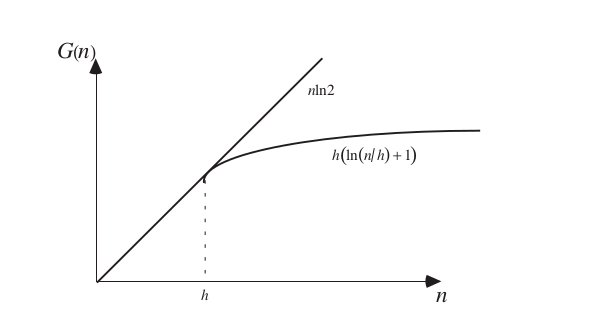
\includegraphics[scale=0.6]{imagenes/funcion_crecimiento_dimension_vc}
	\label{funcion_crecimiento_dimension_vc}
	\caption{Comportamiento de la función de crecimiento \cite[p.~107]{cherkassky_learning_2007}}
\end{figure}

Como podemos ver el comportamiento una vez que el tamaño de la muestra alcanza la dimensión VC converge de forma mucho más rápida.

Hasta ahora no hemos definido formalmente la dimensión VC pero hemos dado una característica de la misma que nos garantiza una buena convergencia. Decimos que un conjunto de funciones indicadoras tiene dimensión VC $h$ si existe una muestra de puntos de tamaño $h$ que puede ser dividida pero no existe una muestra de tamaño $h+1$ que cumpla dicha condición. Es decir, podemos decir que la dimensión VC es la máxima dimensión para la que existe una solución óptima a nuestro problema de dividir el conjunto de datos entre datos anómalos y normales.

Veamos esto con un ejemplo gráfico:

\begin{figure}[H]
	\centering
	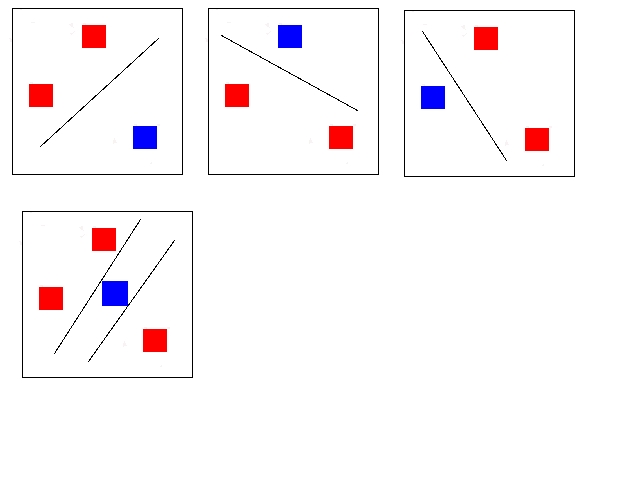
\includegraphics[scale=0.35]{imagenes/dimension_vc}
	\label{dimension_vc}
	\caption{Ejemplo de cálculo de dimensión VC \href{https://commons.wikimedia.org/wiki/File:Vc_linear.jpg}{Wikimedia}}
\end{figure}

Como podemos ver si estamos considerando funciones lineales para aproximar podemos dividir todas las posibilidades con tamaño de muestra 3, pero no con tamaño de muestra 4 por lo que en este caso concreto la dimensión VC será 3.

Ahora podemos volver a la cadena de desigualdades que hemos visto en la sección anterior y actualizarla con la nueva mejor cota que hemos desarrollado con la dimensión VC:

$$H(n)\leq H_{ann}(n) \leq G(n) \leq h(1+\ln (\frac{n}{h}))$$

La definición que hemos dado es para funciones indicadoras pero no para funciones reales en general, vamos a generalizar por tanto la definición de la dimensión de Vapnik-Chervonenkis para el caso de funciones reales.

Consideramos como hemos hecho anteriormente funciones de pérdida del tipo $Q(z,\omega)$ pero acotadas superior e inferiormente por constantes:

$$A\leq Q(z,\omega) \leq B$$

Para este caso podemos pensar en una función indicadora que nos diga si $Q(z,\omega)$ está por encima o por debajo de un cierto valor $\beta$ con $A\leq \beta \leq B$. Podemos por tanto generalizar la dimensión VC para el caso de funciones de pérdida reales como la dimensión VC de este tipo de funciones indicadoras dependientes del parámetro $\beta$.

\subsection{Límites de la generalización}

Venimos de discutir las propiedades de convergencia y consistencia del principio inductivo ERM. Ahora bajo este principio vamos a intentar ir un paso mas allá en la generalización e intentar responder a las siguientes dos preguntas:

\begin{enumerate}
	\item ¿Cómo de cerca están el error real $R(\omega^*)$ y el mínimo error empírico $R_{emp}(\omega^*)$?
	\item ¿Cómo de cerca están el error real $R(\omega^*)$ y el mínimo error posible $R(\omega_0) = \min_{\omega} R(\omega)$?
\end{enumerate}

Estas preguntas las vamos a resolver en el marco que hemos introducido, con todos los conceptos anteriores de la teoría de Vapnik-Chervonenkis en el caso del problema de clasificación binaria que es el que más se ajusta a nuestro problema.

Según Vapnik-Chervonekis se puede acotar el error real cometido por el error empírico con una probabilidad de al menos $1-\eta$ usando el principio inductivo ERM. La cota que hallaron es la siguiente:

$$R(\omega) \leq R_{emp} \omega) + \frac{\epsilon}{2} \biggl( 1+\sqrt{1+\frac{4\cdot R_{emp}(\omega)}{\epsilon}} \biggl)$$

donde:

$$\epsilon = a_1 \cdot \frac{h(\ln (\frac{a_2 n}{h})+1) - \ln (\frac{\eta}{4})}{n}$$

cuando el conjunto de funciones de pérdida $Q(z, \omega)$ contiene un número infinito de elementos, en caso contrario:

$$\epsilon = 2\frac{\ln (N) - \ln (\eta)}{n}$$

y los valores $a_1 , a_2$ son constantes sobre los que se exigen condiciones.

Para empezar según la demostración de Vapnik, los valores $a_1$ y $a_2$ deben estar en los rangos $0<a_1 \leq 4$ y $0<a_2 \leq 2$ siendo la pareja de valores $a_1 = 4$ y $a_2 = 2$ la correspondiente al peor de los casos, dando en como resultado el siguiente valor de $\epsilon$:

$$\epsilon = 4\frac{h(\ln (\frac{2n}{h})) - \ln (\frac{\eta}{4})}{n}$$

Con esta desigualdad estamos dando la cota de cómo se comporta el error real con respecto al error empírico. Podemos ver que, en el mejor de los casos el error real y el error empírico se van a diferenciar en al menos $\frac{\epsilon}{2}$.

Además, para resolver la segunda de las preguntas la teoría de Vapnik-Chervonenkis nos da la siguiente cota con probabilidad al menos $1-2\eta$:

$$R(\omega_n^*)-\min_{\omega} R(\omega) \leq \sqrt{\frac{-\ln (\eta)}{2n}} + \frac{\epsilon}{2} (1+\sqrt{1+\frac{4}{\epsilon}})$$

En este caso podemos ver que la cota es aún mayor que en el caso anterior, teniéndose tanto en esta cota como en la anterior que a mayor nivel de confianza (menor valor de $\eta$) mayor es la cota y por tanto menos información tenemos. Es decir, no podemos conocer una buena cota con un nivel de confianza alto. Este hecho no debería de sorprendernos pues seguimos trabajando con un número finito de datos y ya sabemos que no podemos obtener una aproximación todo lo buena que queramos con un número finito de datos de entrenamiento.

Este hecho también se refleja en los valores analíticos que hemos dado. Pensemos en un escenario con $\eta \rightarrow 0$, es decir un alto nivel de confianza. Entonces si miramos la expresión de $\epsilon$ podemos observar que $-\ln (\frac{\eta}{4})\rightarrow \infty$ y por tanto $\epsilon \rightarrow \infty$ con lo que la cota no nos aportaría ninguna información en ninguno de los dos casos.

Por otro lado si lo que crece es el tamaño de la muestra, es decir, $n\rightarrow \infty$, estamos aumentando el conocimiento que tenemos sobre el problema y por tanto lo razonable sería que ambas cotas tendieran al valor óptimo. En efecto si observamos el valor de $\epsilon$ cuando $n\rightarrow \infty$ vemos que tiende a $0$ por lo que el error empírico y real están muy cerca y de igual forma el error real y el mínimo error posible. Por tanto podemos decir que nuestro nivel de certeza depende del tamaño de la muestra. Este hecho fue visto por Vapnik en su teoría y propuso como valor aproximado de la confianza de la desigualdad aquel que lleva asociado el valor:

$$\eta = \min (\frac{4}{\sqrt{n}},1)$$

\subsection{Principio de minimización del error estructural (SRM)}

Hemos visto una construcción en base al principio inductivo ERM y hemos razonado que funciona bien para casos en los que la proporción $\frac{n}{h}$, es decir la proporción del tamaño de la muestra y la dimensión VC, es grande. En este caso quiere decir que tenemos muchos datos comparado con la dimensión VC y por tanto $\epsilon \approx 0$. Por contra cuando tenemos que $\frac{n}{h}$ es pequeño no tenemos mucha información de la cota. Por tanto, al estar el número de datos fijo por el problema, tenemos que buscar un conjunto de funciones para aproximar la salida del sistema que nos den una dimensión VC controlable para hacerla más o menos grande.

El principio inductivo que pretende plasmar esta idea es el principio de minimización del error estructural o SRM. Bajo este principio se le otorga a la clase de funciones de pérdida de una estructura, es decir, tenemos subconjuntos de la forma $S_k = \{ Q(z,\omega), \ \omega \in \Omega_k \}$ de forma que:

$$S_1 \subset S_2 \subset ... \subset S_k \subset ...$$

donde cada subconjunto de funciones de pérdida tiene asociada una dimensión VC $h_k$ teniéndose el orden:

$$h_1 \leq h_2 \leq ... \leq h_k \leq ...$$

Al igual que en el Teorema clave de la Teoría del Aprendizaje de Vapnik-Chervonenkis se exigía que las funciones de pérdida estuvieran acotadas en este caso vamos a pedir que las funciones contenidas en cada uno de los $S_k$ o bien estén acotadas o si no que cumplan que:

$$\sup_{\omega \in \Omega_k} \frac{(\int Q^p (z,\omega)dp(z))^{\frac{1}{p}}}{\int Q(z,\omega)dp(z)}\leq \tau_k , \ p>2$$

para alguna pareja $(p,\tau_k)$.

En cuanto a la definición del SRM hay dos estrategias prácticas que se llevan a cabo para su implementación que son:

\begin{enumerate}
	\item Mantener la dimensión VC fija y minimizar el error empírico.
	\item Mantener el error empírico constante y pequeño y minimizar la dimensión VC.
\end{enumerate}

Estas implementaciones realmente quedan muy libres en la práctica y se proponen por tanto diferentes estructuras de minimización del error empírico y la dimensión VC que se saben que funcionan bien.

Por tanto este principio no se basa meramente en el buen ajuste de los datos, si no que además pretende hacer una minimización de la complejidad del modelo propuesto.

\subsection{Aproximaciones de la dimensión VC}

Como hemos estado viendo las cotas que hemos expuesto y desarrollado dependen en mayor o menor medida de la dimensión VC. Como es lógico este valor no es fácil de calcular, y de hecho sólo se sabe para unos cuantos conjuntos de funciones de aproximación. Vapnik propuso una método para poder estimar este valor y así poder obtener unas cotas aproximadas.

El procedimiento propuesto por Vapnik consiste en, dadas dos muestras $Z_n^1 , Z_n^2$ de tamaño $n$ de pares $z_i = (x,y)$ de datos de entrada y salida del sistema vamos a medir el error empírico con nuestro modelo que cometemos observando la máxima desviación de los ratios de error de estas dos muestras independientes, es decir:

$$\xi (n) = \max_{\omega} (|Error(Z_n^1) - Error(Z_n^2|)$$

donde $Error(Z_n^i)$ es la tasa de error empírico cometido por el modelo. De acuerdo con la teoría desarrollada por Vapnik-Chervonenkis tenemos que $\xi (n)$ está acotada:

$$\xi (n) \leq \Phi (\frac{n}{h})$$

donde $h$ es la dimensión VC y:

\[ \Phi (\tau) = 
\begin{cases}
1 & si \ \tau <0.5 \\
a\frac{\ln (2\tau) + 1}{\tau - k} \bigg( \sqrt{1+\frac{b (\tau - k)}{\ln (2\tau) + 1}} + 1 \bigg) & en \ otro \ caso
\end{cases}
\]

donde $\tau = \frac{n}{h}$ y las constantes $a = 0.16$ y $b = 1.2$ son constantes estimadas empíricamente por Vapnik y $k = 0.14928$ tomada así para que $\Phi (0.5) = 1$ de forma que la cota sea muy ajustada.

Por tanto describió con esto el siguiente esquema de obtención de la aproximación de la dimensión VC:

\begin{enumerate}
	\item Generamos una muestra de tamaño $2n$ etiquetada $z_{2n}$
	\item Dividimos la muestra en dos del mismo tamaño $Z_n^1$ y $Z_n^2$
	\item Invertir las etiquetas de $Z_n^2$
	\item Mezclar los dos conjuntos de nuevo y entrenar el modelo
	\item Separar el conjunto en dos de nuevo e invertir las etiquetas del segundo, volver a mezclarlos y entrenar de nuevo el modelo
	\item Medir  la diferencia de los errores $\xi (n) = |Error(Z_n^1) - Error(Z_n^2)|$
\end{enumerate}

Como hemos dicho antes la desigualdad $\xi (n) \leq \Phi (\frac{n}{h})$ es muy ajustada y por tanto, podemos obtener la aproximación de $h$ como:

$$h^* = arg \min_{h} [\xi (n) - \Phi (\frac{n}{h})]$$

Es decir, el valor que haga dicha diferencia menor, es decir que más acerque los valores $\xi (n)$ y $\Phi (\frac{n}{h})$.